\chapter{Конструкторская часть}
	\section{Разработка алгоритмов}
На рисунках \ref{fig:classic}, \ref{fig:vino}, \ref{fig:optvino} представлены схемы алгоритмов трёх алгоритмов умножения матриц.

\begin{figure}[H]
	\centering
	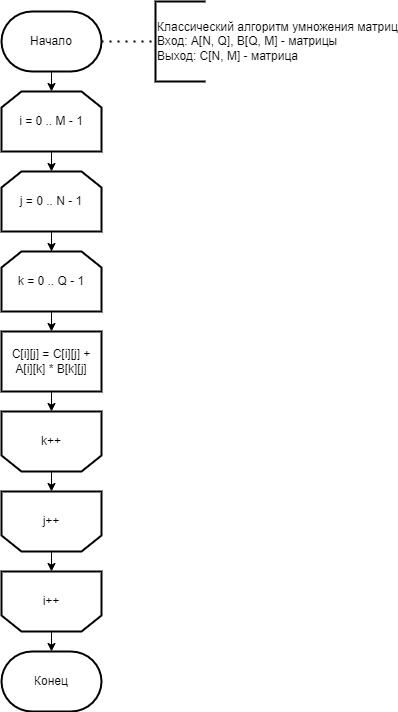
\includegraphics[width=0.7\linewidth]{inc/img/classic}
	\caption{Классический алгоритм}
	\label{fig:classic}
\end{figure}

\begin{figure}[H]
	\centering
	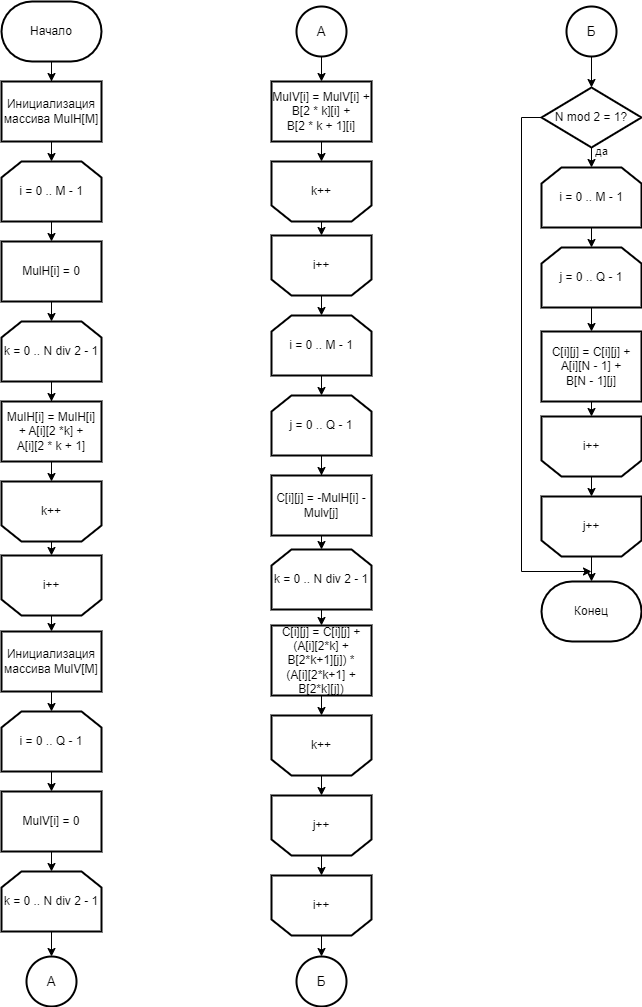
\includegraphics[scale=0.6]{inc/img/vino}
	\caption{Алгоритм Винограда}
	\label{fig:vino}
\end{figure}

\begin{figure}[H]
	\centering
	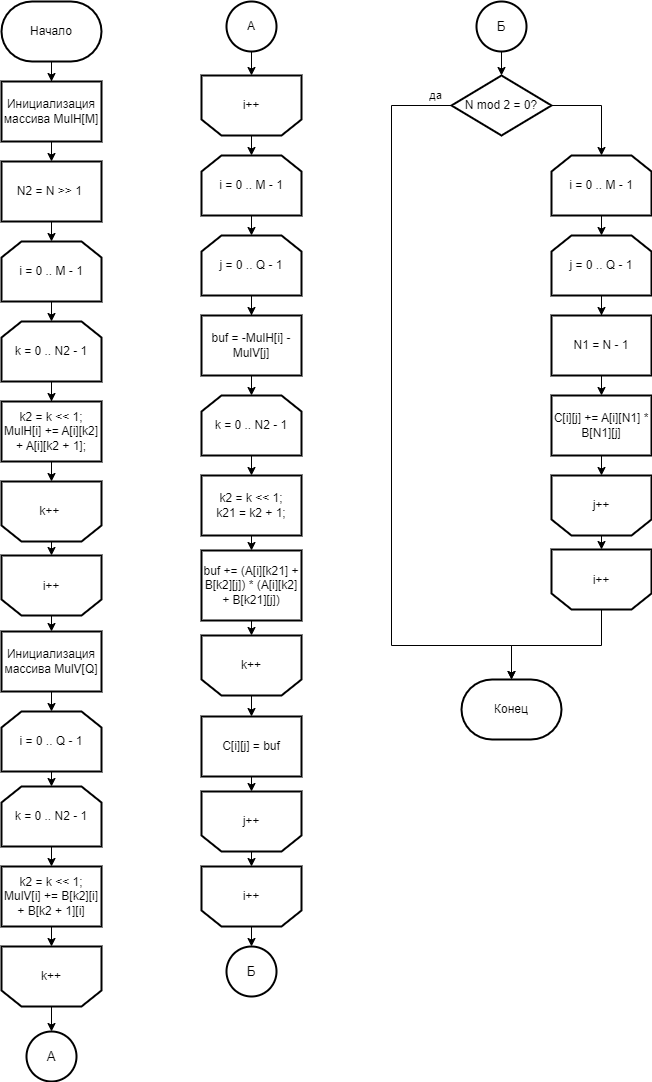
\includegraphics[scale=0.55]{inc/img/optvino}
	\caption{Оптимизированный алгоритм Винограда}
	\label{fig:optvino}
\end{figure}



\section{Оценка трудоёмкости}
Пусть даны две матрицы $A$ и $B$ размерностью $M\times N$ и размерностью $N \times Q$ соответственно. Рассмотрим трудоемкость трёх алгоритмов умножения матриц.

\subsection{Классический алгоритм}
Данный алгоритм был рассмотрен на семинарских занятиях, его трудоемкость равна:
\begin{equation}
	\label{complex_classic}
	f_{classic} = 13MNQ + 4MQ + 4M + 1
\end{equation}

\subsection{Алгоритм Винограда}
Трудоёмкости составных частей алгоритма:
\begin{itemize}
	\item цикл создания вектора MulH $f_{I} = \frac{15}{2}MN + 4M + 2$;
	\item цикл создания вектора MulV  $f_{II} = \frac{15}{2}NQ + 4Q + 2$;
	\item основной цикл $f_{III} = 13MNQ + 4MQ + 4M + 2$;
	\item условный переход при чётном $N$ $f_{IV} = 2$;
	\item условный переход и цикл при нечётном $N$ $f_{IV} = 17MQ + 4M + 4$.
\end{itemize}

Общая трудоемкость алгоритма.

	При чётном $N$.
	\begin{equation}
		\label{vin_even}
		\begin{array}{cc}
			f_{vin} = f_{I} + f_{II} + f_{III} + f_{IV} = 13MNQ + \frac{15}{2}MN +\\ \frac{15}{2}NQ + 4MQ + 8M + 4Q + 8
		\end{array}
	\end{equation}

	При нечётном $N$.
	\begin{equation}
		\label{vin_odd}
		\begin{array}{cc}
			f_{vin} = f_{I} + f_{II} + f_{III} + f_{IV} = 13MNQ + \frac{15}{2}MN +\\ \frac{15}{2}NQ + 21MQ + 12M + 4Q + 10
		\end{array}
	\end{equation}

\subsection{Оптимизированный алгоритм Винограда}
Трудоёмкости составных частей алгоритма:
\begin{itemize}
	\item цикл создания вектора MulH $f_{I} = \frac{13}{2}MN + 2M + 3$;
	\item цикл создания вектора MulV  $f_{II} = \frac{13}{2}NQ + 2Q + 3$;
	\item основной цикл $f_{III} = \frac{19}{2}MNQ + 11MQ + 3M + 1$;
	\item дополнительный цикл при нечётном $N$ $f_{IV} = 11MQ + 2M + 3$;
	\item дополнительный цикл при чётном $N$ $f_{IV} = 2$.
\end{itemize}

Общая трудоемкость алгоритма.

	При чётном $N$.
	\begin{equation}
		\label{complex_vin_even}
		\begin{array}{cc}
			f_{opt} = f_{I} + f_{II} + f_{III} + f_{IV} = \frac{19}{2}MNQ + \frac{13}{2}MN + \frac{13}{2}NQ +\\ 11MQ + 5M + 2Q + 9
		\end{array}
	\end{equation}

	При нечётном $N$.
	
	\begin{equation}
		\label{complex_vin_odd}
		\begin{array}{cc}
			f_{opt} = f_{I} + f_{II} + f_{III} + f_{IV} = \frac{19}{2}MNQ + \frac{13}{2}MN + \frac{13}{2}NQ +\\ 22MQ + 7M + 2Q + 10
		\end{array}
	\end{equation}

\section{Список оптимизаций алгоритма Винограда}
Алгоритм Винограда был оптимизирован с помощью следующих модификаций.
\begin{enumerate}
	\item Замена конструкций вида a = a + b (трудоёмкость = 2) на a += b (трудоёмкость = 1).
	\item Предвычисление некоторых слагаемых.
	\item Замена умножения на 2 (трудоёмкость 2) на побитовый сдвиг (трудоёмкость 1).
\end{enumerate}

\section*{Вывод}

Были разработаны схемы всех трех алгоритмов умножения матриц. Для каждого из них были рассчитаны трудоемкости.


